\chapter{Konzept}
\label{ch:concept}
Die Algorithmen und Prozesse einer Filialplanung spiegeln sehr gut einen allgemeinen Anwendungsfall moderner GIS. 
Neben einer einfachen Hintergrundkarte sind die Mitarbeiter auf Zeichenwerkzeuge, Geo-Daten-Anzeige, thematische Karten und Kennzahlen Berechnungen angewiesen, um akkurate und fundierte Prognosen und Planungen treffen zu können.
Viele theoretische Konzepte und Prozesse passieren hierbei im Hintergrund und sind nicht direkt ersichtlich.


In den folgenden Kapiteln werden Prozesse der Standortanalyse beschrieben und der Fokus auf das Gravitationsmodell von Huff als Algorithmus zur Bestimmung des Marktanteils gelegt.
Ebenso wird die daraus entstehende Architektur des Prototyps vorgestellt.
\section{Algorithmen und Prozesse}
Die Filialplanung ist ein Prozess, der sich aus mehreren Teilprozessen zusammensetzt. 
Einer dieser Teilprozesse ist die Standortanalyse bezogen auf Filialen.
Die Wahl eines Standortes ist keinesfalls immer eindeutig und anhand des potenziellen Umsatzes der neuen Filiale zu erkennen.
So kann es zum Beispiel durchaus sinnvoll sein eine Filiale trotz möglicher Kannibalisierung anderer eigener Filialen dennoch zu eröffnen, weil dies gleichzeitig zu Umsatzeinbußen bei Konkurrenzfilialen führt. 
Der eigene Marktanteil und Gesamtumsatz ist der entscheidende Faktor bei der Filialplanung.
Durch die Anwendung ausgewählter Algorithmen gilt es also folgende Leitfrage zu beantworten:

Wo befindet sich der ideale Standort, um eine neue Filiale zu eröffnen?

Um diese Frage fundiert beantworten zu können, ergeben sich mehrere vorliegende Fragen:

Wo kann ich überhaupt eine neue Filiale eröffnen?

Was ist mit meinen Konkurrenten, was ist mit Kannibalisierung meiner eigenen Filialen?

Wie kann ich folglich also sicherstellen, dass sich mein Gesamtumsatz durch die Neueröffnung steigert?\\

Die Suche nach dem idealen Standort beginnt zunächst bei der Eingrenzung möglicher Standorte.
Im modernen Stadtbild ist die Anzahl freier Standorte begrenzt.
Meist bestimmt das Angebot die Möglichkeiten.

Existiert nun eine Liste möglicher Standorte, muss für jeden Standort der Einfluss auf das bestehende Filialnetz erfasst werden.
Das bestehende Netz kann nur eigene Filialen beinhalten, um die Kannibalisierung meines eigenen Netzes durch eine Neueröffnung zu analysieren, oder Konkurrenzfilialen und Lager einschliessen, um den Einfluss auf den Gesamtmarkt zu berechnen.

Wichtige Parameter für die Berechnung des Marktanteils der Filialen im Netz sind Attraktivität, Nähe zu Zielgruppen und die Entfernung zu anderen Filialen.

Über das Huff-Modell kann die Marktanteil-Auswirkung aller Standorte berechnet werden.
Im Folgenden wird das Modell und zugehörige Komponenten im Detail vorgestellt.



Um eine realistische Abbildung der Welt auf eine Karte zu bringen benötigt es eine Umrechnung eines Ovales, quasi der Erdkugel, auf eine Rechteck, im Fall eines Web-Gis des Bildschirms. 
\subsection{Gravitationsmodell}
\label{subsec:gravitationmodel}
Das \textit{Huff-Modell} (engl. Huff Gravitation Model) ist ein mathematisches Modell zur Abgrenzung und Segmentierung von Marktgebieten \cite{Roy2004}.
Das Modell bestimmt die Wahrscheinlichkeit, mit der Kunden einen Standort (Filiale, Einkaufszentrum) in Abhängigkeit von Distanz und Attraktivität aufsuchen. 
Die Formel wird im allgemeinen wie folgt dargestellt:

\begin{figure}
	\centering
	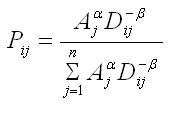
\includegraphics[]{resources/images/huff_model.jpg}
	\caption{Formel des Huff-Modells}
	\label{img:huff_formula}
\end{figure}

Die Wahrscheinlichkeiten werden nun auf der Karte als Punkte dargestellt, die rund um den Standort platziert werden. 
Die Punkte der selben Wahrscheinlichkeiten werden zu Isowahrscheinlichkeitslinien verbunden. 
So entstehen zu jedem Standort verschiedene Gravitationsebenen, die farblich gekennzeichnet werden. 
Die Beeinflussung der verschiedenen Gravitationsebenen führt zu mehreren Farbverläufen, die ein komplexes Bild der Standort Landschaft bilden.
In seiner einfachsten Form berücksichtigt das Modell nur die Distanz und eine simple Kennzahl der Attraktivität (zum Beispiel in Form eines Rankings) für die Wahrscheinlichkeitsberechnung. 
Hierzu wird zunächst ein maximaler Einflussbereich der Filialstandorte definiert. 
Dieser Bereich stellt die Grundlage der Berechnungen dar und muss deswegen bekannt und mit berechenbaren Kennzahlen gefüllt sein.
Zur Bestimmung des Bereiches können einfache geografische Abstände oder Gebiete benutzt werden, wie zum Beispiel eine Berechnung auf Grundlage Berlins als Einflussbereichs.
Vor Allem aber kommen zeitliche oder örtliche Parameter zum Einsatz.
So macht es aus wirtschaftlicher Sicht viel mehr Sinn das Gebiet anhand von Fahrzeitzonen zu berechnen.
So würde ein potenzieller Kunde aus Brandenburg wahrscheinlich auch in einer Filiale in Berlin einkaufen gehen, wenn diese attraktiver, örtlich näher oder besser zu erreichen ist.
Berechnet wird also ein Einzugsbereich, um die Filiale herum.
Ob dies nun eine maximale Fahrtzeit von 30 Minuten ist oder eher eine maximale Distanz von 30 Kilometern, ist auf die einzelne Filiale oder den gewählten Standard der Berechnung zurückzuführen.

Um die Huff-Formel korrekt kalibrieren zu können, genauer gesagt die Parameter alpha und beta empirisch bestimmen zu können, müssen folgende Schritte befolgt werden:

\begin{itemize}
	\item Abgrenzung des Erhebungsgebiets
	\item Unterteilung des Erhebungsgebiets in Untergebiete
	\item Zentroiden der Gebiete festlegen
	\item Alle konkurrierende Einrichtungen identifizieren und Koordinaten erfassen
	\item Entfernungen zwischen den Zentroiden aller Gebiete und aller Einrichtungen berechnen
	\item Spezifizieren aller Eigenschaften zur Kundenbeeinflussung
	\item Wirtschaftliche, soziale und demografische Daten für Gebiete angeben
	\item Studie durchführen für die Frequenz in welcher Kunden Einrichtungen besuchen
\end{itemize}

Weiterführend muss bestimmt werden wie und ob sich das Potenzial über den Verlauf der Distanz des Einzugsbereiches verändert.
Bleibt das Potenzial konstant, würde dies bedeuten die Kunden in den äußeren Bereichen des Gebiets kommen mit der gleichen Wahrscheinlichkeit in die Filiale wie die Kunden in den unmittelbar angrenzenden Bereichen.
Aber gegenteilig wäre ein linear abnehmendes Potenzial wahrscheinlich ebenso nicht vollständig realitätsgetreu, da Kunden ab einer Distanz, die zu groß für den Fuß-Weg wäre, eher das Auto oder den öffentlichen Nahverkehr wählen und dann eventuell direkt zu einer attraktiveren Filiale weiter weg fahren würden. 
Daher kann als grundlegende Distanzfunktion quasi eine beliebig komplizierte Formel gewählt werden.
Aus Gründen der Vereinfachung und Demonstration wird für den Prototyp eine einfache linear abnehmende Distanzfunktion gewählt.

Nachdem nun zunächst die Potenzialberechnung für eine einzelne Filiale anhand der beschriebenen Parameter und Funktionen erfolgen konnte gilt es nun das Potenzial in einem bestehendem Filialnetz zu berechnen.
Als Ergebnis wird hierbei eine Wahrscheinlichkeitsberechnung für sämtliche Filialen des Netzes erwartet, sodass jedem Feld des summierten Gesamt-Einzugsgebietes einen Wahrscheinlichkeitswert zugeordnet werden kann, der beeinflusst von sämtlichen anderen Filialen des Netzes, für jede Filiale des Netzes unterschiedlich sein kann und dementsprechend eingefärbt werden kann.
Das Endergebnis zeigt somit die beschriebene farbliche Gravitationskarte.
\newpage

\section{Architektur}
Die Architektur der Anwendung ergibt sich hauptsächlich aus den fachlichen Anforderungen und technischen Voraussetzungen. 

Das Diagramm \ref{img:components_diagram} zeigt die Komponenten der Anwendung im Zusammenspiel in einer eigenen Darstellung.

\begin{figure}[H]
	\makebox[\textwidth][c]{
	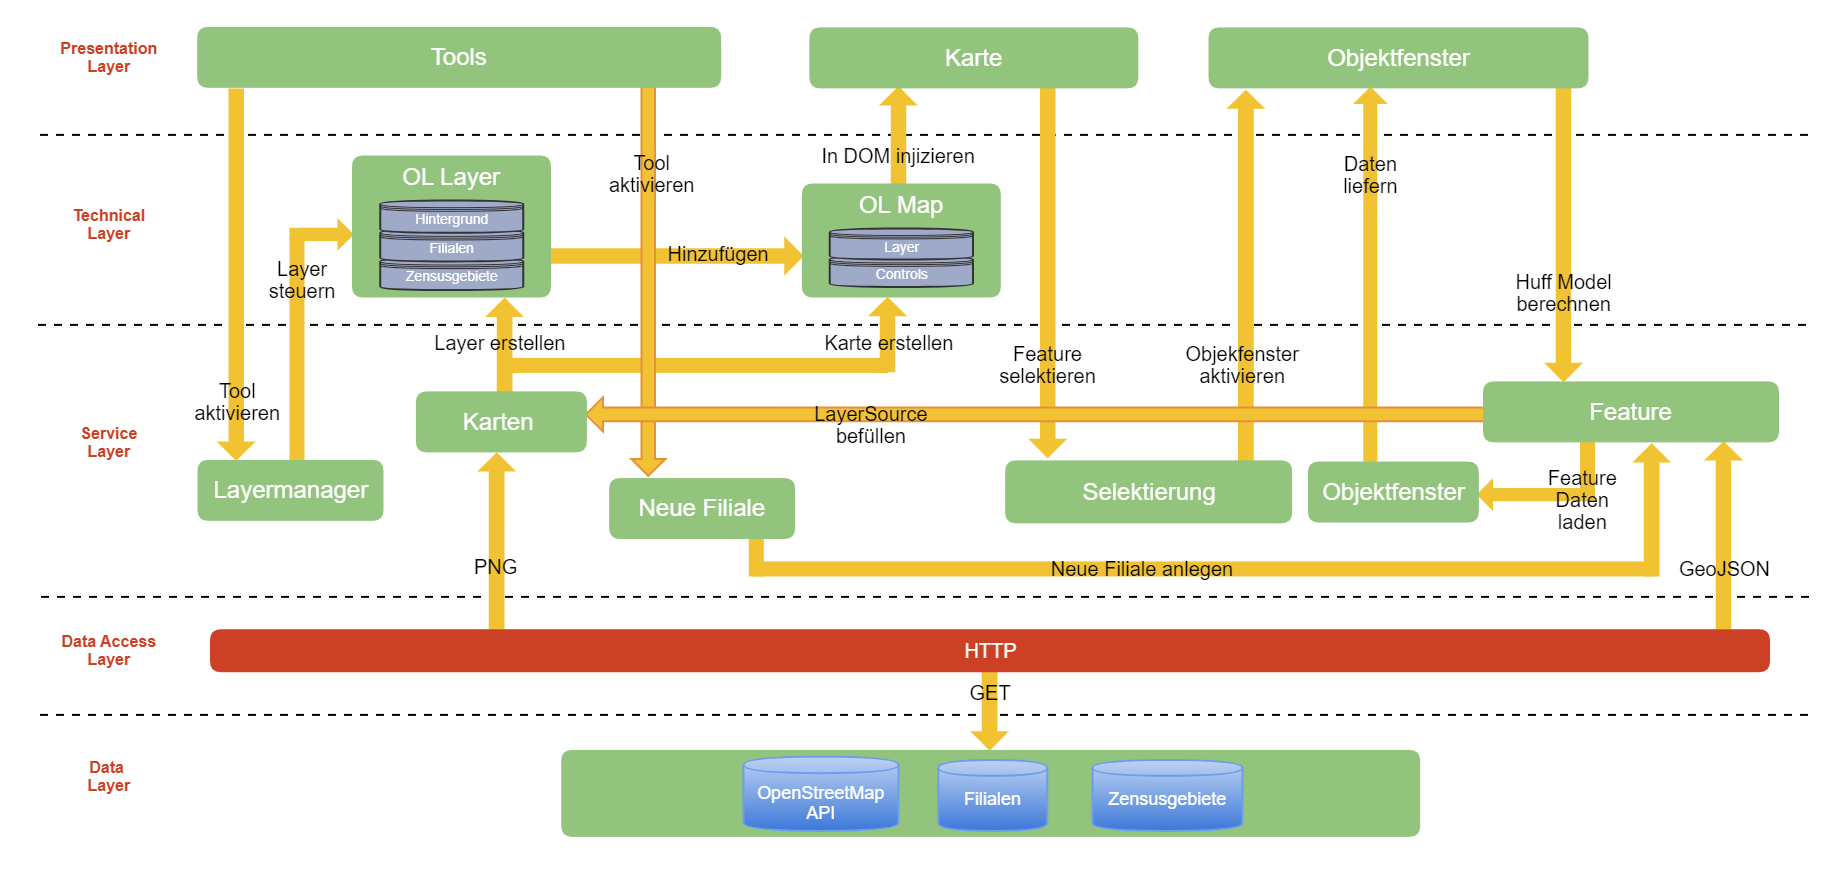
\includegraphics[width=1.0\textwidth]{resources/images/architecture.png}}
	\caption{Komponentendiagramm der Anwendung in eigener Darstellung}
	\label{img:components_diagram}
\end{figure}

Die Anwendung baut im wesentlichen auf vier Komponentengruppen auf:

\begin{itemize}
\item Angular Komponenten
\item Angular Services
\item OpenLayers Karte und Layer
\item Geo-Daten
\end{itemize}

OpenLayers als GIS-Software bildet hierbei den Kern in Form der Karte.
Die Karte bietet an sich bereits einen großen Teil der GIS-Werkzeuge, die für die Anwendung benötigt werden.
Die Karte stellt die Layer und deren Sourcen in der richtigen Projektion dar und bietet die Selektierungs-Interaktion der einzelnen Features.
Sie sorgt also dafür, dass die ovale Weltkarte auf den flachen Bildschirm projiziert wird und der Klick auf eine Pixel-Koordinate des Bildschirmes umgerechnet eine geografische Koordinate widerspiegelt.
Die Karte wird in der Anwendung im BaseMap-Service mit Parametern erstellt und in der OpenLayersMap-Komponente in den DOM injiziert. 

Der Karte werden drei Layer hinzugefügt:

\begin{itemize}
\item Hintergrund-Layer
\item Filial-Layer
\item Zensusgebiete-Layer
\end{itemize}

Fachlich betrachtet kann der Hintergrund-Layer auch als Hintergrundkarte bezeichnet werden, technisch ist er jedoch ebenso ein Layer wie die Filialen und Gebiete. 
Die Layer werden im BaseMap-Service erstellt und der Karte in der OpenLayersMap-Komponente hinzugefügt.
Zu den Layern gehören entsprechende Sources, über die Features in den Layer und somit dargestellt werden können.

Der Hintergrund-Layer ist ein Kachel-Layer (Englisch: Tile-Layer).
Der Layer wird durch ein Gitter (Englisch: Grid) in einzelne Kacheln eingeteilt, die alle einzeln mit Bildern befüllt werden.
Dies ist ein Optimierungsschritt, der den Datentransfer reduziert sowie die Renderingzeit und -performance verbessert.
Die Kachelbilder werden über Http-Requests an die OpenStreetMap-API geladen.

Die beiden Feature-Layer der Filialen und Gebiete sind Vektor-Layer (Englisch: Vector-Layer).
Die jeweiligen Sources der Layer lesen die Features über lokale GeoJSON-Dateien im Feature-Service ein und befüllen den Layer im BaseMap-Service mit den Sourcen.

Nun sind die Features über ihre Layer auf der Karte zu sehen und können über eine Selektions-Interaktion in der Karte ausgewählt werden.
Über den SelectFeature-Service wird daraufhin das Objektfenster aktiviert, welches Informationen über das Feature enthält und die Berechnung des Huff-Modells für die selektierte Filiale starten kann.
Die Daten des Features werden über den Objektfenster-Service in das Objektfenster injiziert.

Über die Tool-Komponente kann eine neue Filiale auf die Karte gesetzt werden und die Layer gesteuert werden.

Sobald eine neue Filiale auf der Karte gesetzt ist wird über den Neue-Filiale-Service ein weiteres Feature in die Filiale-LayerSource geladen und über das Objektfenster kann nun die Berechnung des Huff-Modells gestartet werden.

Über das LayerManager-Tool kann im LayerManager-Service die Sichtbarkeit und Reihenfolge der Layer gesteuert werden.
